\documentclass[10pt]{article}

\usepackage[utf8]{inputenc}
\usepackage[a4paper, lmargin=3cm, rmargin=3cm, tmargin=3cm, bmargin=2.8cm]{geometry}
% \usepackage{charter}
\usepackage{mathpazo}
% \usepackage{newcent}
\usepackage{amsmath}
\usepackage{amssymb}
\usepackage{amsthm}
\usepackage{ifthen}
\usepackage{paralist}
\usepackage{dsfont}
\usepackage{graphicx}
\usepackage[UKenglish]{babel}
\usepackage{epigraph}
\usepackage{bbm}
\usepackage{todonotes}
\usepackage[title, titletoc]{appendix}
\usepackage{titlesec}
\usepackage{etoolbox}
\usepackage{tocloft}
\usepackage[normalem]{ulem}
\usepackage{fancyhdr}
\usepackage{caption}
\usepackage{textcomp}
\usepackage{booktabs}
% \usepackage{parskip}  % uncomment to remove paragraph indents
%\usepackage{refcheck}

% We don't want to see subsections of the appendices in the ToC
\appto\appendices{\addtocontents{toc}{\protect\setcounter{tocdepth}{1}}}
\appto\listoffigures{\addtocontents{lof}{\protect\setcounter{tocdepth}{1}}}
\appto\listoftables{\addtocontents{lot}{\protect\setcounter{tocdepth}{1}}}
\addtocontents{toc}\protect\setcounter{tocdepth}{2}

% Make bullets a little smaller
\renewcommand\labelitemi{$\vcenter{\hbox{\footnotesize$\bullet$}}$}

% Set up hyperlinks. Blue seems to be the only non-sucky default colour.
%\definecolor{DarkBlueLinks}{RGB}{10,85,145}
\definecolor{DarkBlueLinks}{RGB}{5,32,144} % more blue, less green

\usepackage{hyperref}
\hypersetup{
    colorlinks=true,
    linkcolor=DarkBlueLinks,
    filecolor=blue,      
    urlcolor=blue,
    citecolor=DarkBlueLinks,
    pdftitle={Margins and Credit Risk on Vega},
  	pdfauthor={D. \v{S}i\v{s}ka},
}

%\usepackage{draftwatermark}
%\SetWatermarkText{DRAFT}
%\SetWatermarkScale{1.2}

% Set reference names for autoref
\addto\extrasUKenglish{
    \renewcommand{\sectionautorefname}{Section}
    \renewcommand{\subsectionautorefname}{Section}
    \renewcommand{\subsubsectionautorefname}{Section}
}

% Auto-linked glossary entries. 
% Format them in dashed underline/italic (uncomment one) to distinguish from other links.

\newtheorem{proposition}{Proposition}

% Add vertical space between paragraphs but not ToC entries
\setlength{\parskip}{0.5em}
\setlength\cftparskip{0 em}

\author{W. Gawlikowicz and D. \v{S}i\v{s}ka\\
\small{\href{witold@vega.xyz}{witold@vega.xyz} and \href{david@vega.xyz}{david@vega.xyz}}}
\title{Perpetual Futures on Vega}

\date{
    \vspace{2em}
    \today\\
    \vspace{0.5em}
    {\footnotesize }
    \vspace{2em}
}



\begin{document}
\thispagestyle{empty} %\cleardoublepage
\pagestyle{plain}
\lhead[{}{}]       {{}{}}
\rhead[{}{}]       {{}{}}
\pagenumbering{gobble}

\maketitle

\tableofcontents
\pagebreak


\pagestyle{fancyplain}
\pagenumbering{arabic}
\rhead{\rightmark}
\lhead{Perpetual futures}
\rfoot{\thepage}
\cfoot{}
\lfoot{This entire document is~\copyright~\the\year, Gobalsky Labs Ltd. All rights reserved.}


\section{Introduction}
Vega protocol is a blockchain built from the ground up for trading derivatives~\cite{vega whitepaper}.
One of the most popular derivatives on centralised exchanges focusing on derivatives of crypto assets are the perpetual futures. 
The aim of this note is to describe how those could work on Vega. 

\section{Price tracking in a theoretical perpetual futures market}

In the simplest setting there is an underlying asset trading somewhere (on a Vega spot market, on an Ethereum constant function market (CFM) on a centralised exchange...) with price $(S_t)_{t\geq 0}$. 

There is a funding interval $\Delta t > 0$ which can be e.g. $8$ hours though we will work with years as our time units in which case $\Delta t = \frac13 \frac1{365.25} = \frac1{1095.75}$.
This gives us a sequence of funding payment dates $t_i := i\Delta t$, $i=0,1,\ldots$.
There is continuously compounding interest rate $r$ (equivalently a risk-free asset that grows at the constant rate $r$).

Moreover there is a market where participants bid to enter into a long or short {\em perpetual futures contract} at a {\em strike} $(F_t)_{t\geq 0}$.  
The contract is perpetual and cannot be terminated. 
However at time $t$ it is possible to go back to the market and trade in the opposite direction (i.e. if long 1 perpetual futures contract then enter a 1 unit short contract and vice-versa) at strike $F_t$.   
If at time $t=0$ two parties agree on strike $F_0$ then:
\begin{enumerate}
\item At $t=0$ no payments are made\footnote{An exchange will expect the parties to deposit margin balance, for now we ignore this}; i.e. the contract has current value $0$.
\item While the contract is in place the long pays the short, at every $t_i$, $i=1,2,\ldots$ the amount $G_i = \frac1{\Delta t}\int_{t_{i-1}}^{t_i} (F_u - S_u) \,du $ i.e. the observed average difference  between the futures market strike and the underlying. 
\item At termination long gets $F_t - F_0$. 
\end{enumerate}  



A simple no-arbitrage argument will show that the strike, which from now on we'll refer to as the perpetual futures price, must track the underlying price. 

Assuming the funding payments are frequent (and thus taking $\Delta t \to 0$) and summing up the payments we see the present value of the funding payment the long side pays is 
\[
\int_0^t e^{-ru} (F_u - S_u)\,du\,.
\]

We thus get a similar result to~\cite{he:fundamentals} on how perpetual future strike and underlying price are related.

\begin{proposition}
\label{prop price tracking}
Assume that the underlying and strike prices are given by some stochastic process $(S_t)_{t\geq 0}$ and $(F_t)_{t\geq 0}$ adapted to a filtration $\mathbb F = (\mathcal F_t)_{t\geq 0}$.



Assume that there is some risk neutral measure under which the underlying is a martingale. 
Let us use $\mathbb E$ to denote expectation under this risk-neutral measure
and assume that the expected discounted value is integrable in the sense that $\mathbb E \int_0^\infty e^{-ru} |S_u|\,du < \infty$ and assume that the strike process satisfies the same i.e. $\mathbb E\int_0^\infty e^{-ru} |F_u|\,du < \infty$. 
Then either there is arbitrage or the current underlying and perp strike prices satisfy 
\[
F_0 = S_0(1+r)\,.
\]
\end{proposition}

\section{Practical considerations}

\subsection{Marking to market}
Rather then waiting until position gets unwound to charge or pay the final cashflow $F_t-F_0$ all position in the market get marked to market
with a predefined frequency (up to the nearest block time) whereby each party gets charged or paid 
the amount $V(F_t-F_{t-\Delta})$, where $V$ is their open volume (negative for shorts), 
$F_t$ is the new mark price on the perpetual futures market, $F_{t-\Delta}$ is the mark price from the last time a given position has been marked-to-market or modified
and $\Delta>0$ is the length of the interval between mark-to-market updates (or position change).

All positions will be automatically managed (a forced closeout may occur) depending on their available collateral and current margin requirements. 
For more details see Section~\ref{sec:funding_in_maintenance}.

\subsection{Exchanging funding payments}\label{sec:funding_payment}

We have three sequences of times: 
\begin{enumerate}
    \item the underlying price sampling times $(u_k)_{k \in \mathbb N}$,
    \item the mark price update times $(s_k)_{k\in \mathbb N}$ and
    \item the funding payment times $(t_k)_{k\in \mathbb N}$.
\end{enumerate}

Heuristically the funding rate at time $t_k$ should be
\[
R_{t_k} = \frac{\text{mark price TWAP} - \text{index TWAP}}{\text{index TWAP}}
\]

So for time $t_{k-1}$ and $t_k$ we want to calculate $G_k$. 

Let $K=\max(j\in \mathbb N : u_j \leq t_{k-1})$ and 
$K^+ = \max(j\in \mathbb N : u_j \leq t_k)$. Let $\Delta u_k = u_{k+1} - u_{k}$ for $k > K$ and $k < K^{+}-1$, let $\Delta u_{K} = u_{K+1} - t_{k-1}$ and $\Delta u_{K^+} = t_k - u_{K^+}$. Then we calculate index TWAP\footnote{time-weighted average price} as:
\[
\hat S_{t_k} = \frac1{t_{K^+} - t_{K}}\sum_{k=K}^{K^+} S_{u_k} \Delta u_k\,\,\,\text{if}\,\,\, K^+ > K\,\,\, \text{and} \,\,\, \hat S_{t_k} = S_{t_K}\,\,\, \text{otherwise}\,.    
\]
Similarly we need to get the mark price TWAP. 
To that end let $L = \max(j\in \mathbb N : s_j \leq t_{k-1})$ and $L^+ = \max(j\in \mathbb N : s_j \leq t_k)$. 
Let $\Delta s_k = s_{k+1} - s_{k}$ for $k > L$ and $k < L^{+}-1$, let $\Delta s_L=s_{L+1}-t_{k-1}$ and $\Delta s_{L^+}=t_k-u_{L^+}$. 
Then the mark price TWAP applicable in the period, which we call $\hat F_{t_k}$, should be:
\[
\hat F_{t_k} = \frac1{s_{L^+} - s_L}\sum_{k=L}^{L^+} F_{s_k} \Delta s_k\,\,\,\text{if}\,\,\, L^+ > L\,\,\, \text{and} \,\,\, \hat F_{t_k} = F_{t_L}\,\,\, \text{otherwise}\,.    
\]
 
At time $t_k$ the long should pay the short the amount
\[
G_{t_k} = \hat F_{t_k} - \hat S_{t_k}   
\]
An alternative way to see the payment is to get it via the funding rate:
\[
G_{t_k} = (\hat F_{t_k} - \hat S_{t_k})\frac{\hat S_{t_k}}{\hat S_{t_k}} = R_{t_k} \hat S_{t_k}\,,\,\,\,\text{where the funding rate is}\,\,\, R_{t_k} = \frac{\hat F_{t_k} - \hat S_{t_k}}{\hat S_{t_k}}\,.
\]
Notice that the choice of the denominator is entirely arbitrary and we could equally well have:

\[
G_{t_k} = (\hat F_{t_k} - \hat S_{t_k})\frac{\hat F_{t_k}}{\hat F_{t_k}} = \tilde R_{t_k} \hat F_{t_k}\,,\,\,\,\text{where the funding rate is}\,\,\, \tilde R_{t_k} = \frac{\hat F_{t_k} - \hat S_{t_k}}{\hat F_{t_k}}\,.
\]


\subsection{Margin considerations}
\label{sec:funding_in_maintenance}
We need to include the estimate of the upcoming funding payment in maintenance margin estimate for the party. 
Let $t_{k-1}$ be the time of the last funding payment. Let $t$ be current time ($t<t_k$). 
Calculate $G_t$ as above by replacing $t_k$ with $t$ everywhere. 
Set 
\[
m^{\text{maint}}_t = \text{slippage part} + F_t \cdot \text{RF} + \text{margin funding factor}\max(0,G_t).    
\]
We have $\text{margin funding factor} \in [0,1]$.
For more details on how the risk factors RF and slippage part are defined see~\cite{margins paper} and~\cite{margins spec}.

\subsection{Ability to replicate properties of existing markets}

After reading through even a small portion of documentation on existing perpetual futures markets across different venues one quickly realises that no such thing as a "canonical perpetual futures contract" exists. 

\subsubsection{Funding payment calculation}
Venues can differ to some extent in various aspects of how $\hat F_{t_k}$ or $\hat S_{t_k}$ are constructed, but perhaps the most stark difference are observed in how the the funding rate is constructed.

A certain modification that particularly stands out is the introduction of a an interest rate component along with a min and max operator so that the funding rate takes form:

$$
R_{t_k} = \frac{\hat F_{t_k} - \hat S_{t_k}}{\hat S_{t_k}} + \min \Bigg (a,\max \bigg(b, \frac{(1+(t_k-t_{k-1})r)\hat S_{t_k} - \hat F_{t_k} }{\hat S_{t_k}} \bigg ) \Bigg ), 
$$
where $a$ and $b$ are constants such that $ a \ge b $ and $r$ is the interest component which may be constant or time-dependent.

\begin{figure}[!htb]
\minipage{0.32\textwidth}
  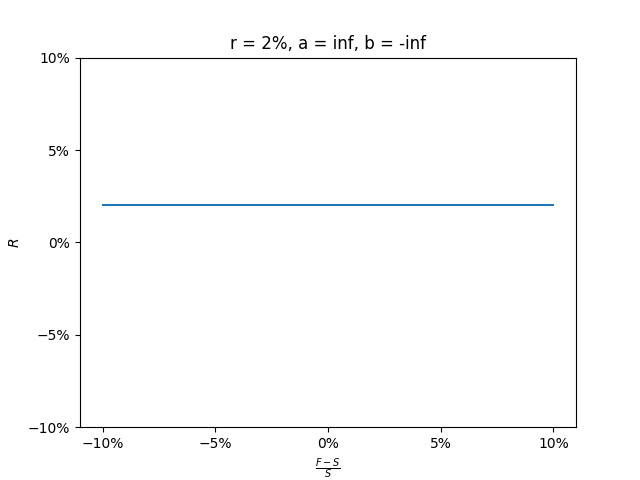
\includegraphics[width=\linewidth]{./plots/r_0.02_a_inf_b_-inf_c_inf_d_-inf_k_1.png}
  \caption{$\\r=2\%,\ a=-b=\infty.$}\label{fig:clamp1}
\endminipage\hfill
\minipage{0.32\textwidth}
  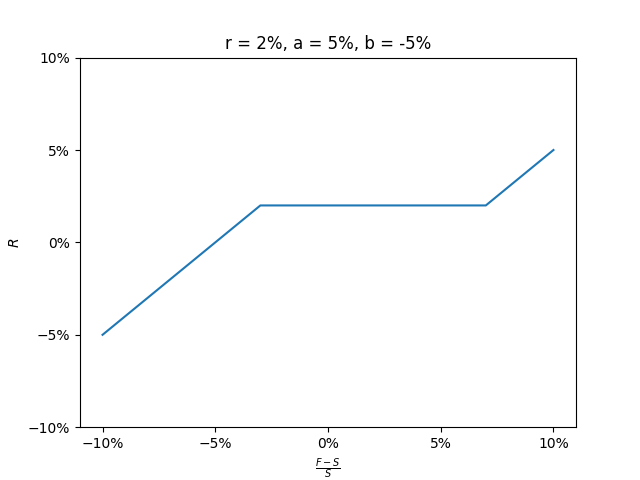
\includegraphics[width=\linewidth]{./plots/r_0.02_a_0.05_b_-0.05_c_inf_d_-inf_k_1.png}
  \caption{$\\r=2\%,\ a=-b=5\%.$}\label{fig:clamp22}
\endminipage\hfill
\minipage{0.32\textwidth}%
  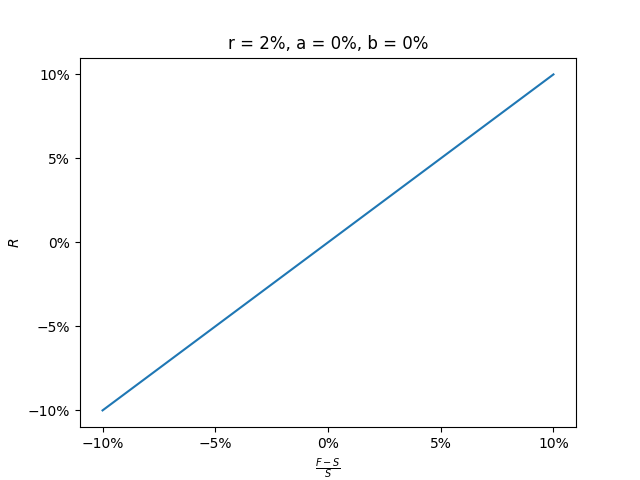
\includegraphics[width=\linewidth]{./plots/r_0.02_a_0_b_0_c_inf_d_-inf_k_1.png}
  \caption{$\\r=2\%,\ a=-b=0\%.$}\label{fig:clamp3}
\endminipage
\end{figure}

Since Vega Protocol strives to offer adequate flexibility to allow community to shape the markets according to its needs we choose to allow reproducing these feature by prescribing the following form for the implementation of the funding payment component described in section ~\ref{sec:funding_payment}. That modified funding payment $\tilde G_{t_k}$ is then:

\begin{equation}\label{eqn:modified_funding_payment}
\tilde G_{t_k} = \hat F_{t_k} - \hat S_{t_k} + \min \Bigg (a\hat S_{t_k},\max \bigg(b\hat S_{t_k}, e^{r_c(t_k-t_{k-1})} \hat S_{t_k} - \hat F_{t_k} \bigg ) \Bigg ), 
\end{equation}

where $r_c$ is the continuous rate of return set for the market (can be updated via governance) and $[t_k,t_{k-1})$ is the time interval in years for which the funding payment is being calculated.

However as the team has not identified any specific use case for the these additional parameters we recommend initially setting $a=b=r_c=0$, unless setting them to different values solves a specific issue identified by the community.

\subsubsection{Funding payment scaling and clamping}

Irrespective of what formulation is chosen for the funding payment it may in some cases be desirable to scale or clamp the resulting figure before calculating the cashflows to be exchanged between parties. Take the funding payment calculated using \eqref{eqn:modified_funding_payment} and denoted $\tilde G_{t_k}$. Then we propose to calculate the funding payment per position of size 1 as:

$$
\bar G_{t_k} = k \min \Big (c\hat S_{t_k},\max \big(d\hat S_{t_k}, \tilde G_{t_k} \big ) \Big )
$$
where $c$, $d$ and $k$ are constants such that $ c \ge d $ and $k\geq 0$.

The constants $c$ and $d$ can be used to set the bounds on the resulting funding rate. While this may reduce the gains of parties expecting the positive funding payment and thus reduce the pressure for the perpetual futures market to move more in line with the underlying spot market it may still be a worthy consideration as it can give parties a bound on the maximum loss they can expect in a funding period. 

The constant $k$ can be used to tune the trading pressure parties with negative funding payments will experience and thus implicitly the responsiveness of the perpetual futures market to the changes in the underlying spot market. It could be useful in scenarios where the market designer wishes to have a certain funding payment frequency while mimicking the aggregate funding payment magnitude of a market with a different funding frequency.

\begin{figure}[!htb]
\minipage{0.32\textwidth}
  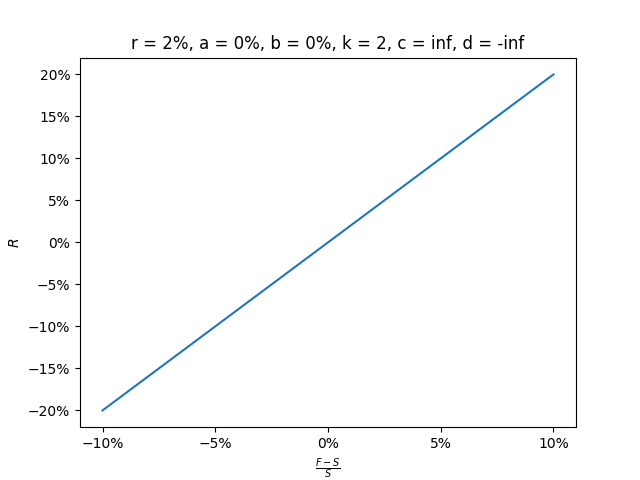
\includegraphics[width=\linewidth]{./plots/r_0.02_a_0_b_0_c_inf_d_-inf_k_2.png}
   \caption{$\\r=2\%,\ a=-b=0,\\ k=2,\ c=-d=0.$}\label{fig:clamp1}
\endminipage\hfill
\minipage{0.32\textwidth}
  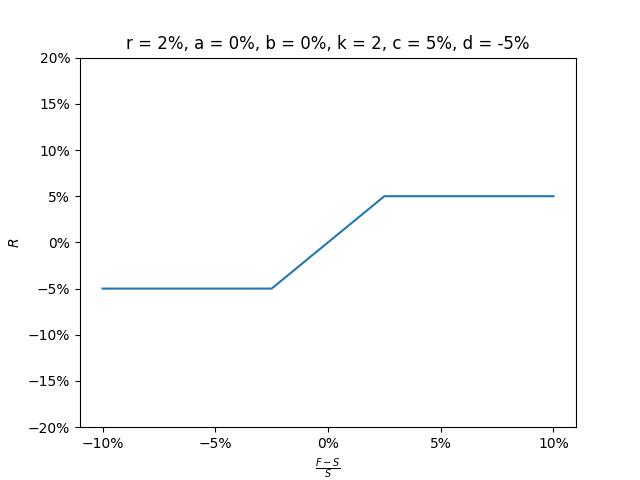
\includegraphics[width=\linewidth]{./plots/r_0.02_a_0_b_0_c_0.05_d_-0.05_k_2.png}
  \caption{$\\r=2\%,\ a=-b=0,\\ k=2,\ c=-d=5\%.$}\label{fig:clamp22}
\endminipage\hfill
\minipage{0.32\textwidth}%
  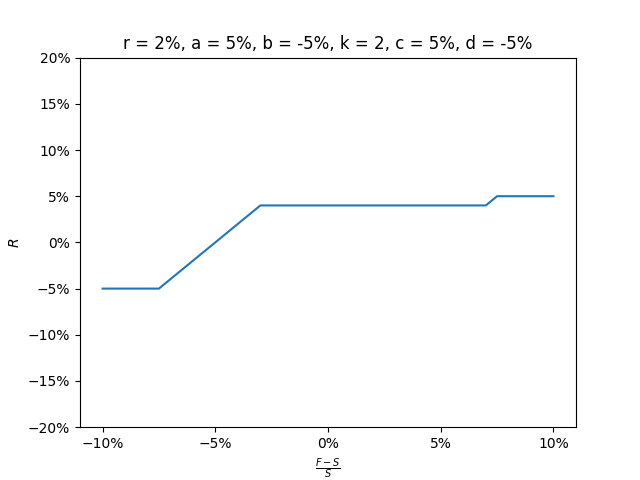
\includegraphics[width=\linewidth]{./plots/r_0.02_a_0.05_b_-0.05_c_0.05_d_-0.05_k_2.png}
  \caption{$\\r=2\%,\ a=-b=5\%,\\ k=2,\ c=-d=5\%.$}\label{fig:clamp3}
\endminipage
\end{figure}

\subsection{Omitted properties}
Some of the properties that can be observed in various venues, but which we deliberately choose not to reproduce are discussed below.

\subsubsection{Tolerance region}

There are venues which use the notion of impact bid and ask price to specify the region within which the differences between $F_{t_k}$ and $S_{t_k}$ are considered negligible and thus not impacting the funding payment. The impact bid/ask price is the average fill price of an order of a fixed notional (called impact notional) at the buy/sell side of the order book. The basic funding payment discussed in section ~\ref{sec:funding_payment} would then take the form:

$$
 \hat G_{t_k} = (\hat F_{t_k} - \hat S_{t_k})\mathbbm{1}_{ (\hat F_{t_k} - \hat S_{t_k}) \notin A },
$$
where
$$
\mathbbm{1}_{ x \notin A } = \begin{cases}
    0 & \text{if } x \in A,\\
    1              & \text{otherwise,}
\end{cases}
$$ 
and $A$ is some interval, say $A=[(1-c)F_{t_k},(1+c)F_{t_k}]$, where $c$ is a constant.


However, we choose not to employ this mechanism in our implementation of the funding rate calculation.
      
\subsubsection{Non-homogeneous time weighting}

Certain venues modify the time-weighted average price used for funding rate calculation to assign different importance to observations depending on their relative time from the funding payment, however we choose not to employ such a mechanism in our implementation of the funding rate calculation.

\subsection{Funding payment and spot sampling frequency}

In this section we will briefly consider the impact of funding frequency and spot sampling frequency on the funding payments observed in a market.

We will use the two curves displayed below alongs with 7 day funding frequency, spot curve sampled every 1 hour and perp curve sampled every 5 minutes as our baseline setup.

\begin{figure}[h]
    \centering
    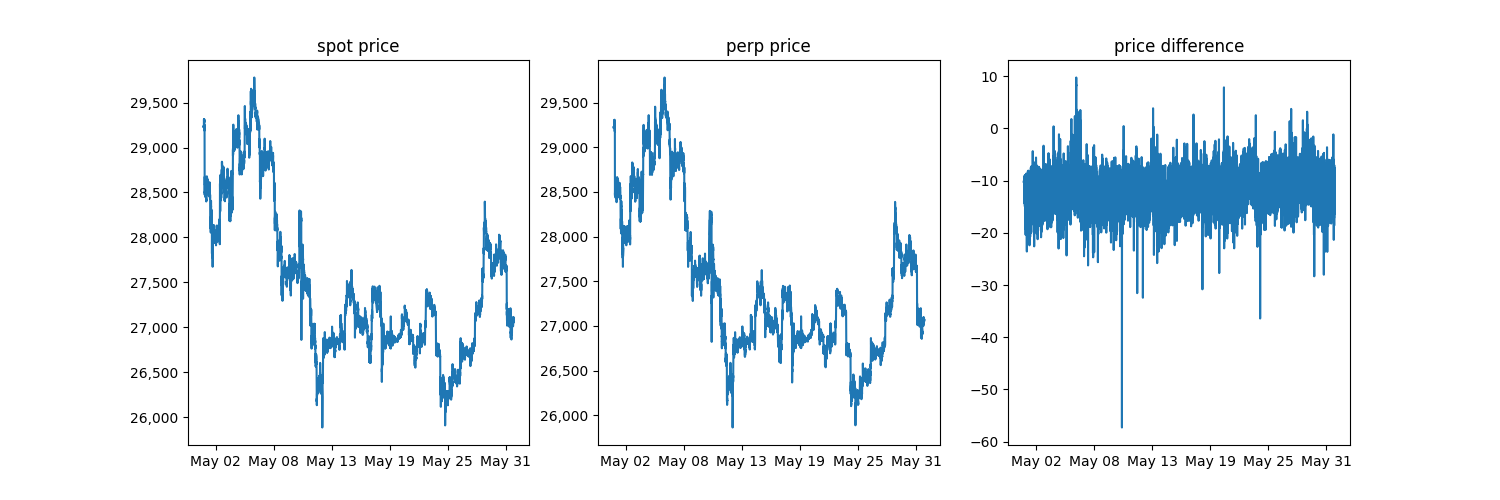
\includegraphics[width=\textwidth]{./plots/example_curves.png}
    \caption{Example BTC/USD spot and perpetual features prices for May 2023.}
    \label{fig:example_curves}
\end{figure}

The resulting funding payments and rate of return for the perpetual contracts of size 1 held throughout such market are displayed in figure ~\ref{fig:resulting_funding_periods}.

\begin{figure}[h]
    \centering
    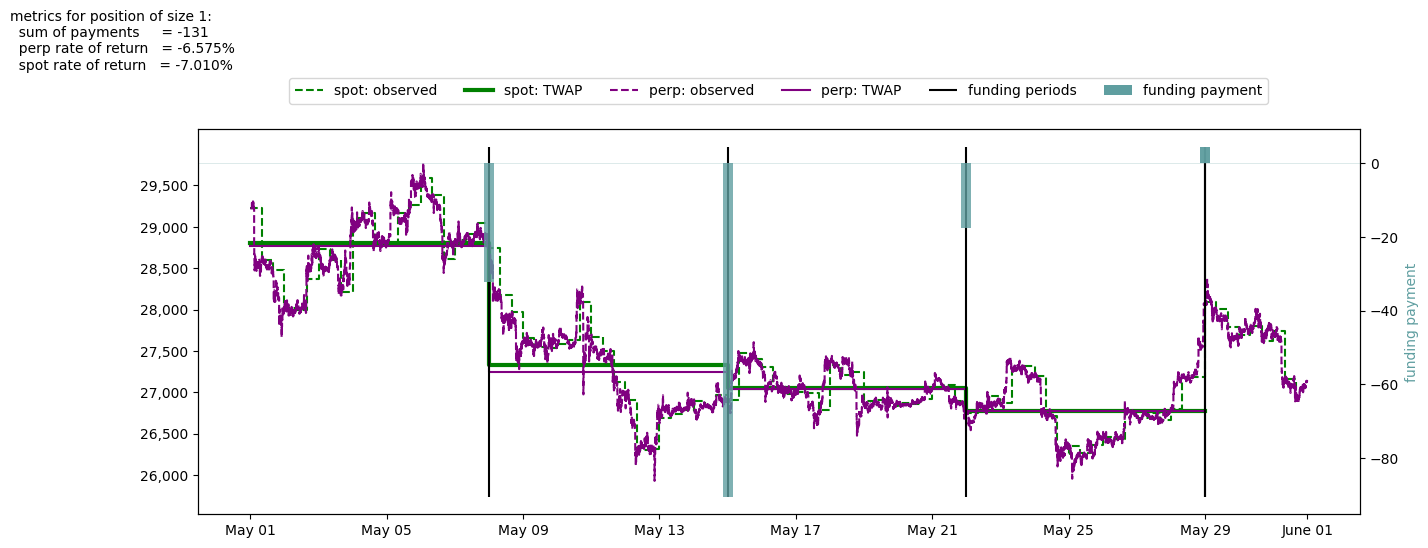
\includegraphics[width=\textwidth]{./plots/7d-payment-frequency_8h-spot-sampling-300s_perp-sampling.png}
    \caption{Resulting funding payments for the baseline case. Interactive version can be found at: \href{https:/github.com/vegaprotocol/research}{https:/github.com/vegaprotocol/research}.}
    \label{fig:resulting_funding_periods}
\end{figure}

The impact of varying the funding payment frequency is summarised in table ~\ref{tbl:funding_frequency}.

\begin{tabular}{llrrr}
\toprule
 & funding_frequency & spot_rr & perp_rr & sum_funding_payments \\
\midrule
0 & 7d & -7.01E-02 & -6.56E-02 & -1.36E+02 \\
1 & 1d & -7.01E-02 & -6.06E-02 & -2.81E+02 \\
2 & 12h & -7.01E-02 & -6.30E-03 & -1.87E+03 \\
3 & 6h & -7.01E-02 & 6.07E-02 & -3.83E+03 \\
4 & 3h & -7.01E-02 & 1.85E-01 & -7.46E+03 \\
5 & 1h & -7.01E-02 & 7.36E-01 & -2.36E+04 \\
6 & 30min & -7.01E-02 & 1.46E+00 & -4.48E+04 \\
7 & 10min & -7.01E-02 & 4.33E+00 & -1.29E+05 \\
8 & 5min & -7.01E-02 & 8.68E+00 & -2.56E+05 \\
\bottomrule
\end{tabular}


The impact of varying the spot sampling frequency is summarised in table ~\ref{tbl:spot_sampling}.

\begin{table}[!htbp]
\caption{Impact of varying spot sampling frequency}
\label{tbl:spot_sampling}
\begin{tabular}{lrr}
\toprule
frequency & perp rate of return & sum of funding payments \\
\midrule
7d & 0.076308 & -4.28E+03 \\
1d & -0.057820 & -3.63E+02 \\
12h & -0.063995 & -1.83E+02 \\
6h & -0.065458 & -1.40E+02 \\
3h & -0.067809 & -7.14E+01 \\
1h & -0.068639 & -4.71E+01 \\
30min & -0.068613 & -4.79E+01 \\
10min & -0.068650 & -4.68E+01 \\
5min & -0.068625 & -4.76E+01 \\
\bottomrule
\end{tabular}
\end{table}


\appendix
\section{Proofs}
\begin{proof}[Proof of Proposition ~\ref{prop price tracking}]
	
\end{proof}

Let us start by noting that our assumptions that $\mathbb E\int_0^\infty e^{-ru} |S_u|\,du < \infty$ and $\mathbb E\int_0^\infty e^{-ru} |F_u|\,du < \infty$ imply that 
\[
\left|\mathbb E \int_0^\infty e^{-rt}(F_t-S_t)\,dt\right| \leq \mathbb E \int_0^\infty e^{-rt}\left|F_t-S_t\right|\,dt \leq \mathbb E \int_0^\infty e^{-rt}|F_t|+|-S_t|\,dt < \infty\,.
\]

Since the parties make no payment upon entering the contract the value at time $0$ must be $0$ and thus we must have for every $t\geq 0$ that
\[
0 = \mathbb E \left[e^{-rt} (F_t-F_0) - \int_0^t e^{-ru}(F_u - S_u)\,du \right]\,.
\]
As the discounted underlying is a martingale we must also have, for every $t\geq 0$, that 
\[
0 = \mathbb E[e^{-rt}S_t - S_0]\,.
\]
Let us write $\psi_t = \mathbb E [e^{-rt}(F_t - S_t)]$. 
Then for every $t\geq 0$ we have  
\[
\psi_t = F_0(e^{-rt} - 1) + \psi_0 + \int_0^t \psi_u\,du\,.
\]
We can solve this integral equation the same way as we would solve an ODE with an integrating factor (i.e. calculate $d(e^{-t} \psi_t)$ and integrate). 
This takes us to 
\[
e^{-t}\psi_t = \psi_0 - r F_0 \int_0^t e^{-u}e^{-ru}\,du\,.
\]
Evaluating the integral we get
\[
e^{-t}\psi_t = \psi_0 - \frac{r F_0}{1+r} (e^{-(1+r)t} - 1)
\]
and so
\[
\psi_t = e^t \psi_0 - \frac{r F_0}{1+r} (e^{-rt} - e^t)\,.
\]
This is 
\[
\mathbb E [e^{-rt}(F_t - S_t)] = e^t(F_0-S_0) - \frac{r F_0}{1+r} (e^{-rt} - e^t)
= e^t\left(F_0 - S_0 - \frac{r F_0}{1+r} \right) - e^{-rt}\frac{r F_0}{1+r}\,.
\]
Let $\gamma = F_0 - S_0 - \frac{r F_0}{1+r}$. 
We see that
\[
\mathbb E \int_0^\infty e^{-rt}(F_t-S_t)\,dt = \gamma \int_0^\infty e^t\,dt - \frac{r F_0}{1+r}\int_0^\infty e^{-rt}\,dt = \gamma \int_0^\infty e^t\,dt - \frac{ F_0}{1+r}\,.
\]
Thus 
\[
\mathbb E \int_0^\infty e^{-rt}(F_t-S_t)\,dt = 
\left\{ 
\begin{split}
+\infty	\,\,\, \text{if}\,\,\, \gamma > 0\,,\\
- \frac{ F_0}{1+r} \,\,\, \text{if}\,\,\, \gamma = 0\,,\\
-\infty	\,\,\, \text{if}\,\,\, \gamma < 0\,.\\
\end{split}
\right.
\]
Note that by assumption we have 
\[
\left|\mathbb E \int_0^\infty e^{-rt}(F_t-S_t)\,dt\right| \leq \mathbb E\int_0^\infty e^{-rt}|F_t-S_t|\,dt \leq \mathbb E\int_0^\infty e^{-rt}|F_t|\,dt + \mathbb E\int_0^\infty e^{-rt}|S_t|\,dt < \infty\,.
\]
But $\left|\mathbb E \int_0^\infty e^{-rt}(F_t-S_t)\,dt\right| < \infty$ means that $\gamma = 0$ which means that 
\[
F_0 = S_0(1+r)\,.
\]





\begin{thebibliography}{10}

\bibitem{he:fundamentals}
S. He and A. Manela and O. Ross and V. von Wachter. Fundamentals of Perpetual Futures. {\em arXiv}:2212.06888, 2023.

%\bibitem{derman:kani:riding} 
%Derman, E. and Kani, I., Riding on a smile, {\em Risk Magazine}, 1994.
%
%\bibitem{dupire:pricing} 
%Dupire, B., Pricing and hedging with smiles, {\em Mathematics of Derivative Securities}, Cambridge Uni. Press 1997.
%
%\bibitem{carr madan}
%P. Carr and D. Madan. Option valuation using the fast Fourier transform.
%{\em J. Comput. Finance}, 2, 61-–73, 1998.
%
%\bibitem{cont tankov}
%R. Cont and P. Tankov. {\em Financial Modelling with Jump Processes}. Chapman \& Hall CRC. 2004.
%
%\bibitem{composing_contracts} 
%S. P. Jones, J.-M. Eber and J. Seward. Composing contracts: an adventure in financial engineering. In: Oliveira J.N., Zave P. (eds) FME 2001: Formal Methods for Increasing Software Productivity. Springer 2001.
%
%\bibitem{glasserman:monte} P. Glasserman. {\em Monte Carlo Methods in Financial Engineering}. Springer 2004.
%
%\bibitem{follmer:schied}
%H. F\"ollmer and A. Schied. {\em Convex and coherent risk measures}.\\ 
%\href{https://www.math.hu-berlin.de/~foellmer/papers/CCRM.pdf}{https://www.math.hu-berlin.de/$\sim$foellmer/papers/CCRM.pdf}, 2008.
%
%\bibitem{broadie:du:moallemi}
%M. Broadie, Y. Du and C. C. Moallemi. Risk Estimation via Regression. {\em Operations Research}, \href{https://doi.org/10.1287/opre.2015.1419}{63(5), 1077--1097}, 2015.
%
%\bibitem{emmbrechts:wang}
%P. Embrechts and R. Wang. {\em Seven proofs for the subadditivity of expected shortfall}.\\
%\href{https://people.math.ethz.ch/~embrecht/ftp/Seven_Proofs.pdf}{https://people.math.ethz.ch/$\sim$embrecht/ftp/Seven\_Proofs.pdf}, 2015.
%
%\bibitem{rnap}
%D. \v{S}i\v{s}ka. {\em Risk-neutral asset pricing}.\\
%\href{http://www.maths.ed.ac.uk/~dsiska/RNAP-Notes.pdf}{http://www.maths.ed.ac.uk/$\sim$dsiska/RNAP-Notes.pdf}, 2017.
%
%\bibitem{mcm}
%D. \v{S}i\v{s}ka. {\em Monte-Carlo methods}.\\
%\href{http://www.maths.ed.ac.uk/~dsiska/MonteCarloMethods.pdf}{http://www.maths.ed.ac.uk/$\sim$dsiska/MonteCarloMethods.pdf}, 2018.
%
%
%\bibitem{belomestny variance}
%D. Belomestny, L. Iosipoi and N. Zhivotovskiy. Variance reduction via empirical variance minimization: convergence and complexity. 
%{\em \href{https://arxiv.org/abs/1712.04667}{arXiv:1712.04667}}, 2017.
%
%\bibitem{giles multilevel nested}
%M. B. Giles and A.-L. Haji-Ali. Multilevel nested simulation for efficient risk estimation. {\em \href{https://arxiv.org/abs/1802.05016}{arXiv:1802.05016}}, 2018.

\bibitem{vega whitepaper}
G. Danezis, D. Hrycyszyn, B. Mannerings, T. Rudolph and D. \v{S}i\v{s}ka. Vega Protocol: A liquidity incentivising trading protocol for smart financial products. {\em \href{https://vega.xyz/papers/}{Vega research paper}}, 2018.

\bibitem{margins paper}
D. \v{S}i\v{s}ka. Margins and Credit Risk on Vega. {\em \href{https://vega.xyz/papers/}{Vega research paper}}, 2019.

\bibitem{margins spec}
Vega protocol specifications. Margin calculator.\\ {\em \href{https://github.com/vegaprotocol/specs/blob/master/protocol/0019-MCAL-margin_calculator.md}{https://github.com/vegaprotocol/specs/blob/master/protocol/0019-MCAL-margin\_calculator.md}}.


%\bibitem{vidales siska szpruch}
%M. Sabate-Vidales, D. \v{S}i\v{s}ka and L. Szpruch. 
%Unbiased Deep Solvers for Linear Parametric PDEs. {\em \href{https://arxiv.org/abs/1810.05094}{arXiv:1810.05094}}, 2018.
%
%\bibitem{siska calibration}
%D. \v{S}i\v{s}ka. Incentives for Model Calibration on Decentralized Derivatives Exchanges: Consensus in Continuum. {\em \href{https://dx.doi.org/10.2139/ssrn.3534272}{SSRN}}, 2020. 

%\bibitem{bjork:arbitrage} T.~Bj\"ork. {Arbitrage Theory in Continous Time}. Oxford University Press, 2009.

%\bibitem{brigo:mercurio}
%D. Brigo and F. Mercurio.  {\em Interest Rate Models - Theory and Practice}, Springer, 2006.

%\bibitem{delbaen:schachermayer} 
%F.~Delbaen and W.~Schachermayer. 
%A general version of the fundamental theorem of asset
%pricing. {\em Math. Ann.} 300(3), 463–520, 1994.

%\bibitem{filipovic:term}
%D.~Filipovic. {\em Term Structure Models}. Springer, 2009.

%\bibitem{gut:intermediate} A. Gut. {\em An Intermediate Course in Probability}. Springer 2009.

%\bibitem{karatzas:shereve:brownian} I.~Karatzas and S. E.~Shreve. {\em Brownian Motion and Stochastic Calculus}. Springer 1991. 

%\bibitem{kolmogorov:fomin:real} A.~N.~Kolmogorov and S.~V.~Fomin.
%{\em Introductory Real Analysis}. Dover, 1975.

%\bibitem{glasserman:monte} P. Glasserman. {\em Monte Carlo Methods in Financial Engineering}. Springer 2004.

%\bibitem{gut:intermediate} A. Gut. {\em An Intermediate Course in Probability}. Springer 2009.

%\bibitem{grimmett:stirzaker:probability} G. Grimmett and D. Stirzaker. {\em Probability and Random Processes}. Third Edition. Oxford University Press 2001.

%\bibitem{oksendal:stochastic} B. {\O}ksendal. {\em Stochastic Differential Equations}. Springer 2003.

%\bibitem{ross:a:first} S. Ross. {\em A First Course in Probability}. Fifth Edition. Prentice--Hall 1998.
%\bibitem{capinski:kopp:measure} M. Capinski and P. E.~Kopp. {\em Measure, Integral and Probability}. Springer 2004.

%\bibitem{grimmett:stirzaker:probability} G. R. Grimmett and D. R.~Stirzaker. {\em Probability and Random Processes}. Oxford University Press 2001.

\end{thebibliography}


\end{document}
